\section{Realisierungsformen}
\begin{center}
	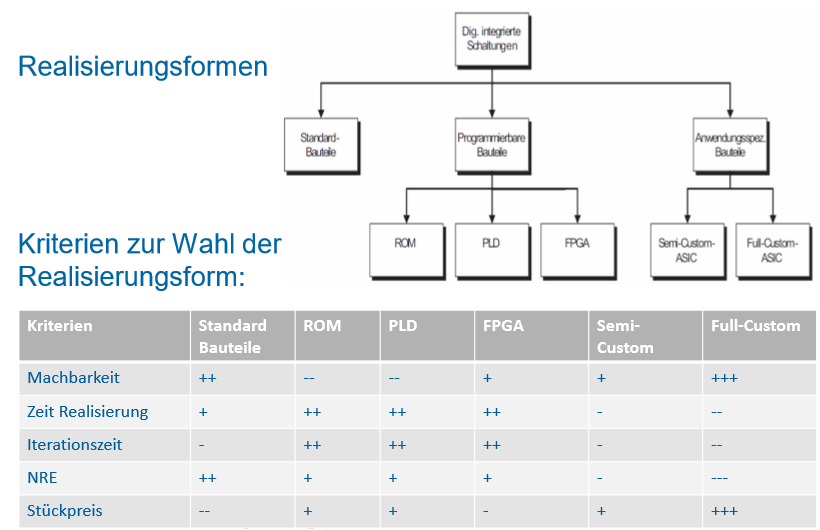
\includegraphics[width=\columnwidth]{Images/realisierungsformen}
\end{center}

\subsection{Standard-Bauelemente}
Komponenten mit fixer Funktion zB USB-Controller, MCU, Gatter etc. Standard-Bauteile werden in grossen Stückzahlen gefertigt. Für komplexere Anwendungen sind jedoch häufig Kombinationen benötigt, was zu einem grösseren PCB führt. Die Kosten sind für NRE sehr gering, können aber auch rasch teuer werden für grössere Stückzahlen. Einsatzgebiet sind Prototypen

\subsection{Programmierbare Bauteile}
\subsubsection{ROM}
Können programmiert werden zB PROM (one time programmable) oder EEPROM (Electrically Eraseable). Die Realisierungszeit ist sehr klein, da einfach der Speicher geändert werden kann. Die Kosten sind relativ gering. Das Einsatzgebiet beschränkt sich jedoch auch Kombinatorischen Schaltungen oder Look-Up-Table (LUT)

\subsubsection{PLD}
Programmable Logic Device verstehet man allgemein programmierbare Bausteine bestehend aus einer AND oder OR Stufe, wovon mindestens eine Stufe programmierbar ist. Für einfach Steueraufgaben sind die Kosten relativ klein. Das Einsatzgebiet wurde jedoch von FPGA fast komplett verdrängt.

\subsection{FPGA}
Field Programmable Gate Array haben ein breites Einsatzgebiet und werden vorallem für das Verarbeiten von grossen Datenmengen zu verarbeiten eingesetzt. Die Kosten sind moderat.

\subsection{ASIC}
Alle Hardware vollständig definierbar und optimiert für Stromverbrauch, Grösse, Funktionalität. Leider sind sehr hohe NRE und langer Designprozess notwendig. Als Anwendung werden diese für alle Extrembereich verwendet.

\subsection{Entwursprozess}
Das y-Modell von DD Gajski beschreibt 3 Sichten mit 5 Hierarchieebenen:
\begin{center}
	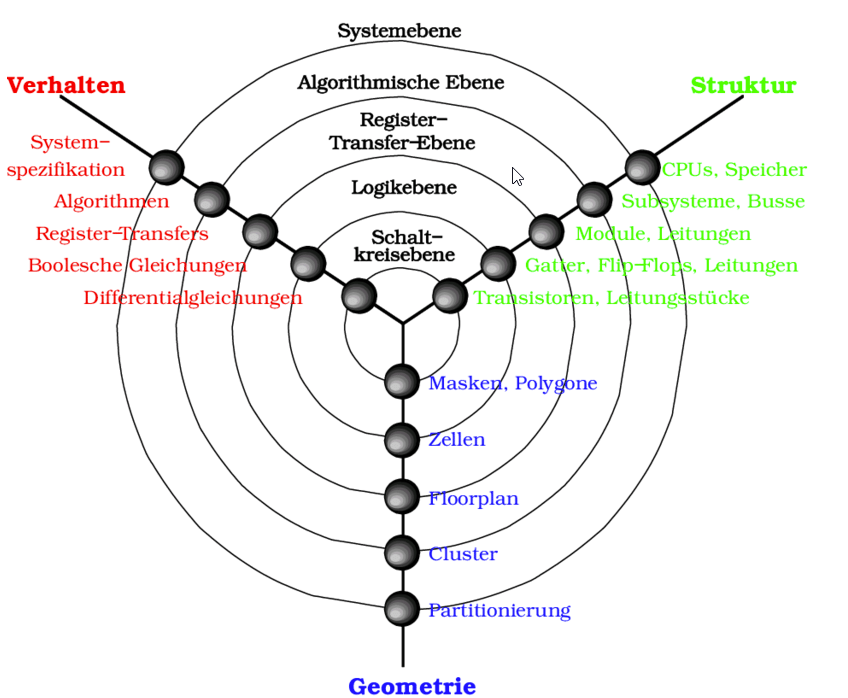
\includegraphics[width=\columnwidth]{Images/y-modell}
\end{center}
 
Der Allgemeine Ablauf fürs das Entwickeln von FPGAs sieht wie folgt aus
\begin{center}
	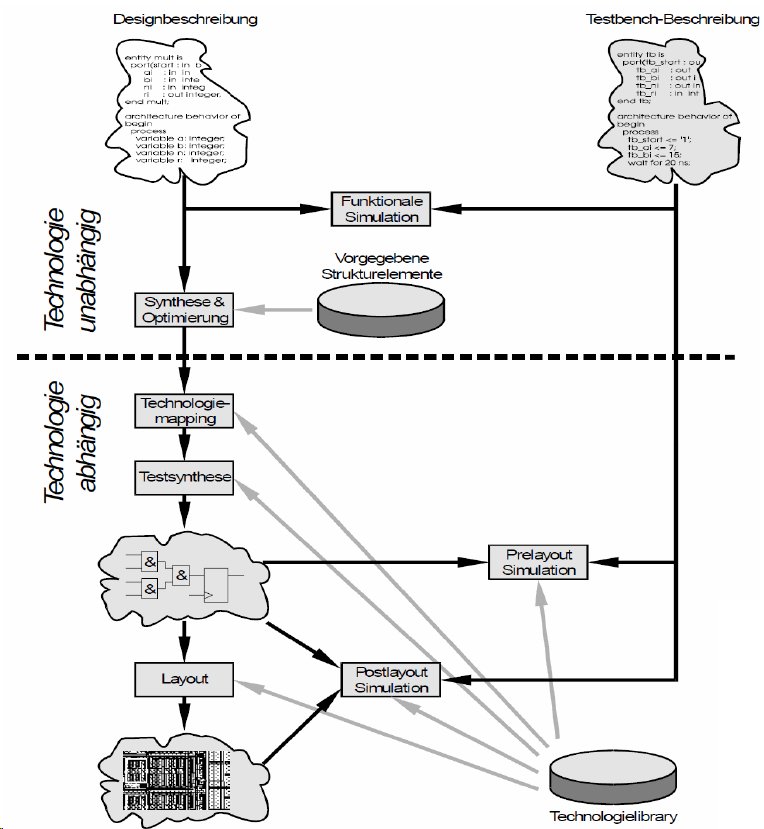
\includegraphics[width=\columnwidth]{Images/ablauf}
\end{center}
Es wird dabei in Frontend (oben), welche Technologie unabhängig ist, und Backend (unten) welche Techonolie abhängig ist unterschieden.